%
% Copyright (c) 2013 The NetBSD Foundation, Inc.
% All rights reserved.
%
% This code is derived from software contributed to The NetBSD Foundation
% by Radoslaw Kujawa.
%
% Redistribution and use in source and binary forms, with or without
% modification, are permitted provided that the following conditions
% are met:
% 1. Redistributions of source code must retain the above copyright
%    notice, this list of conditions and the following disclaimer.
% 2. Redistributions in binary form must reproduce the above copyright
%    notice, this list of conditions and the following disclaimer in the
%    documentation and/or other materials provided with the distribution.
%
% THIS SOFTWARE IS PROVIDED BY THE NETBSD FOUNDATION, INC. AND CONTRIBUTORS
% ``AS IS'' AND ANY EXPRESS OR IMPLIED WARRANTIES, INCLUDING, BUT NOT LIMITED
% TO, THE IMPLIED WARRANTIES OF MERCHANTABILITY AND FITNESS FOR A PARTICULAR
% PURPOSE ARE DISCLAIMED.  IN NO EVENT SHALL THE FOUNDATION OR CONTRIBUTORS
% BE LIABLE FOR ANY DIRECT, INDIRECT, INCIDENTAL, SPECIAL, EXEMPLARY, OR
% CONSEQUENTIAL DAMAGES (INCLUDING, BUT NOT LIMITED TO, PROCUREMENT OF
% SUBSTITUTE GOODS OR SERVICES; LOSS OF USE, DATA, OR PROFITS; OR BUSINESS
% INTERRUPTION) HOWEVER CAUSED AND ON ANY THEORY OF LIABILITY, WHETHER IN
% CONTRACT, STRICT LIABILITY, OR TORT (INCLUDING NEGLIGENCE OR OTHERWISE)
% ARISING IN ANY WAY OUT OF THE USE OF THIS SOFTWARE, EVEN IF ADVISED OF THE
% POSSIBILITY OF SUCH DAMAGE.
%
% 
\documentclass[dvipsnames,table]{beamer}
\usepackage{polski}

\usetheme{Rochester}
\usecolortheme{orchid}

\usepackage{listings}
\usepackage{ucs}
\usepackage[utf8x]{inputenc}
\usepackage{wasysym}
\usepackage[normalem]{ulem}
\usepackage{amsmath}
\usepackage{hyperref}

\setbeamertemplate{navigation symbols}{}
\setbeamertemplate{caption}[numbered]
\setbeamerfont{caption}{size=\scriptsize}
\setbeamercolor{framenote}{bg=NetBSD-orange!25}
\setbeamercolor{rednote}{bg=Red!25}
\setbeamercolor{palette primary}{use=structure,fg=white,bg=NetBSD-orange}
\setbeamercolor{palette secondary}{use=structure,fg=white,bg=NetBSD-orange2}

\setbeamertemplate{itemize item}{\scriptsize\raise1pt\hbox{\donotcoloroutermaths$\blacktriangleright$}}
\setbeamertemplate{itemize subitem}{\tiny\raise1pt\hbox{\donotcoloroutermaths$\bullet$}}
\setbeamertemplate{itemize subsubitem}{\tiny\raise1pt\hbox{\donotcoloroutermaths{--}}}

\setbeamertemplate{enumerate item}{\insertenumlabel.}
\setbeamertemplate{enumerate subitem}{\insertenumlabel.\insertsubenumlabel}
\setbeamertemplate{enumerate subsubitem}{\insertenumlabel.\insertsubenumlabel.\insertsubsubenumlabel}
\setbeamertemplate{enumerate mini template}{\insertenumlabel}

\setbeamercolor{itemize item}{fg=NetBSD-orange, bg=NetBSD-orange}
\setbeamercolor{itemize subitem}{fg=NetBSD-orange, bg=NetBSD-orange}
\setbeamercolor{itemize subsubitem}{fg=NetBSD-orange, bg=NetBSD-orange}

\setbeamercolor{section number projected}{fg=white,bg=NetBSD-orange}
\setbeamercolor{subsection number projected}{fg=white,bg=NetBSD-orange}
\setbeamercolor{button}{bg=NetBSD-orange,fg=white}

\setbeamertemplate{section in toc}[circle]
\setbeamertemplate{subsection in toc}[square]


\definecolor{NetBSD-orange}{RGB}{242,103,17}
\definecolor{NetBSD-orange2}{RGB}{177,76,12}
\hypersetup{colorlinks=true,linkcolor=white,urlcolor=NetBSD-orange}

\setlength{\tabcolsep}{8pt}
\renewcommand{\arraystretch}{1.2}

\newcommand{\nbsdcolor}[1] {
	{\color{NetBSD-orange} #1}
}

\lstset{
   language=C,
   basicstyle=\tiny,
   breaklines=true,
   escapechar=\@,
   commentstyle=\color{NetBSD-orange}
}

\AtBeginSection[]{
\frame{\sectionpage}
}

\title{System operacyjny NetBSD\\ w zastosowaniach wbudowanych}


\author{Radoslaw Kujawa -- rkujawa@NetBSD.org}

\institute{The NetBSD Foundation}

\begin{document}

\begin{frame}
\titlepage
\end{frame}

\begin{frame}[allowframebreaks]
\frametitle{Spis treści}
{
\hypersetup{colorlinks=true,linkcolor=black,urlcolor=NetBSD-orange}
\tableofcontents
}
\end{frame}

\section{Garść informacji na temat NetBSD}

\begin{frame}
\frametitle{Czym jest NetBSD?}
\begin{itemize}
	\item UNIX-owy system operacyjny
	\item ...
\end{itemize}
\end{frame}

\begin{frame}
\frametitle{Historia NetBSD w pigułce}
\begin{itemize}
	\item Projekt NetBSD istnieje od 20 lat, wywodzi się z Berkeley Software Distribution -- systemu operacyjnego rozwijanego w grupie CSRG na Uniwersytecie w Berkeley
	\item Korzenie systemu sięgają kodu oryginalnego UNIXa - prawie pół wieku historii

\end{itemize}
\end{frame}

\begin{frame}
\frametitle{Kto obecnie używa NetBSD?}
\begin{itemize}
	\item Powszechnie znane firmy oraz organizacje
	\begin{itemize}
		\item Apple - AirPort Extreme, Time Capsule, różne komponenty OS X oraz iOS
		\item Blackberry/RIM - Stos IP, sterowniki, pkgsrc w systemie QNX
		\item Dell - \href{http://www.dell.com/us/business/p/force10-ftos/pd}{Force10 OS}
 		\item Microsoft - Architektura \href{http://research.microsoft.com/en-us/projects/emips/}{eMIPS}
		\item NASA - International Space Station
		\item oraz inni
	\end{itemize}
	\item Hobbyści
	\item Hakerzy
	\item Naukowcy
	\item Uniwersytety
\end{itemize}
\end{frame}

\begin{frame}
\frametitle{Kto pracuje nad NetBSD?}
\begin{itemize}
	\item Niezależni developerzy zrzeszeni w fundacji NetBSD
	\item Firmy - w ramach kontraktów
	\begin{itemize}
		\item Semihalf (PL)
		\item Denx Software Engineering (DE)
		\item 3am Software Foundry (US)
	\end{itemize}
\end{itemize}
\end{frame}


\begin{frame}
\frametitle{Cechy NetBSD}
\begin{itemize}
	\item Małe wymagania sprzętowe
	\item Bardzo dobra przenośność -- 57 portów, 12 architektur CPU

	\item Przykładanie uwagi do ,,czystości'' projektu oraz implementacji
	\item W zgodzie z duchem UNIXa

	\item Powyższe cechy czynią NetBSD doskonałą platformą dla rozwiązań wbudowanych
\end{itemize}
\end{frame}

% co jest system wbudowany, cechy systemu wbudowanego
% granica miedzy sprzetem ogolnego przeznaczenia a systemami wbudowanymi sie zaciera

\begin{frame}
\frametitle{Jądro NetBSD}
\begin{itemize}
	\item Klasyczny kernel monolityczny z modułami\footnote{Systemy wbudowanie zwykle nie korzystają z modułów.}
	\item Wymaga jednostki zarządzania pamięcią (MMU)

\end{itemize}
\end{frame}

\section{Budowa aplikacji wbudowanych na NetBSD}

\begin{frame}
\frametitle{Od czego zacząć?}
\begin{itemize}
	\item Pomysł
\end{itemize}
\end{frame}	


\begin{frame}
\frametitle{Sprzęt do rozwoju aplikacji wbudowanych}
\begin{itemize}
	\item Łatwo dostępne zestawy uruchomieniowe i ewaluacyjne
	\begin{itemize}
		\item Raspberry Pi
		\item Beagleboard, Beaglebone
		\item Pandaboard
		\item wiele innych

	\end{itemize}
	\item Możliwość wykorzystania niektórych produktów ,,z półki'' jako zestawu
	\begin{itemize}
		\item NAS oparte o PowerPC MPC824x - znane produkty firm Synology, QNAP (sandpoint)
		\item Linksys NSLU2 (evbarm)
		\item Nokia N900 (evbarm)
		\item oraz inne
	\end{itemize}
\end{itemize}
\end{frame}

\begin{frame}
\frametitle{Budowanie NetBSD ze źródeł}
\begin{itemize}
	\item Procedura budowania jest trywialna
	\begin{itemize}
		\item \tt{cvs co src \&\& cd src \&\& cvs up -dP}
		\item \tt{./build.sh -m [port] tools}
		\item \tt{./build.sh -m [port] distribution}
	\end{itemize}
	\item Skrypt build.sh jest tylko opakowauje standardowe pliki Makefile
	\item Kompilacja wskrośna całego systemu możliwa z prawie każdego innego systemu UNIX-owego (Linux, MacOS X, *BSD, Solaris, itd.)
\end{itemize}
\end{frame}


\begin{frame}
\frametitle{Wybór platformy sprzętowej}
\begin{itemize}
	\item Czy architektura procesora (powerpc, arm, mips, ...) jest już obsługiwana? 
	\item Czy platforma, którą chcę wykorzystać jest już obsługiwana?
	\item Czy wszystkie peryferia są obsługiwane?
	\item ,,port''
	\item Dzięki modularnej architekturze NetBSD przeniesienie systemu na nową platformę, czy dodanie wsparcia dla nowego typu procesora jest wzlgędnie proste
	\item Ale dalej nie jest to zadanie dla nowicjusza
\end{itemize}
\end{frame}

\section{Prosta aplikacja wbudowana}

\begin{frame}
\frametitle{Beaglebone}

\begin{columns}[c]
\column{3in}

\begin{itemize}

	\item SoC Texas Instruments AM335x 720MHz
	\item ARM Cortex-A8 (ARM v7)
	\item 256MB DDR2
	\item Slot micro SD, Ethernet, host USB
	\item Ustandaryzowane złącza pozwalają na dołączanie dodatkowych modułów (,,cape'' jak ,,shield'' w Arduino)
	\item Interfejsy typowe dla mikrokontrolerów - SPI, I\textsuperscript{2}C, ADC, CAN, itd.
	\item Teraz dostępna nowa wersja ,,Black'' - 1GHz, 512MB DDR3 (\$45)
\end{itemize}

\column{1.5in}
	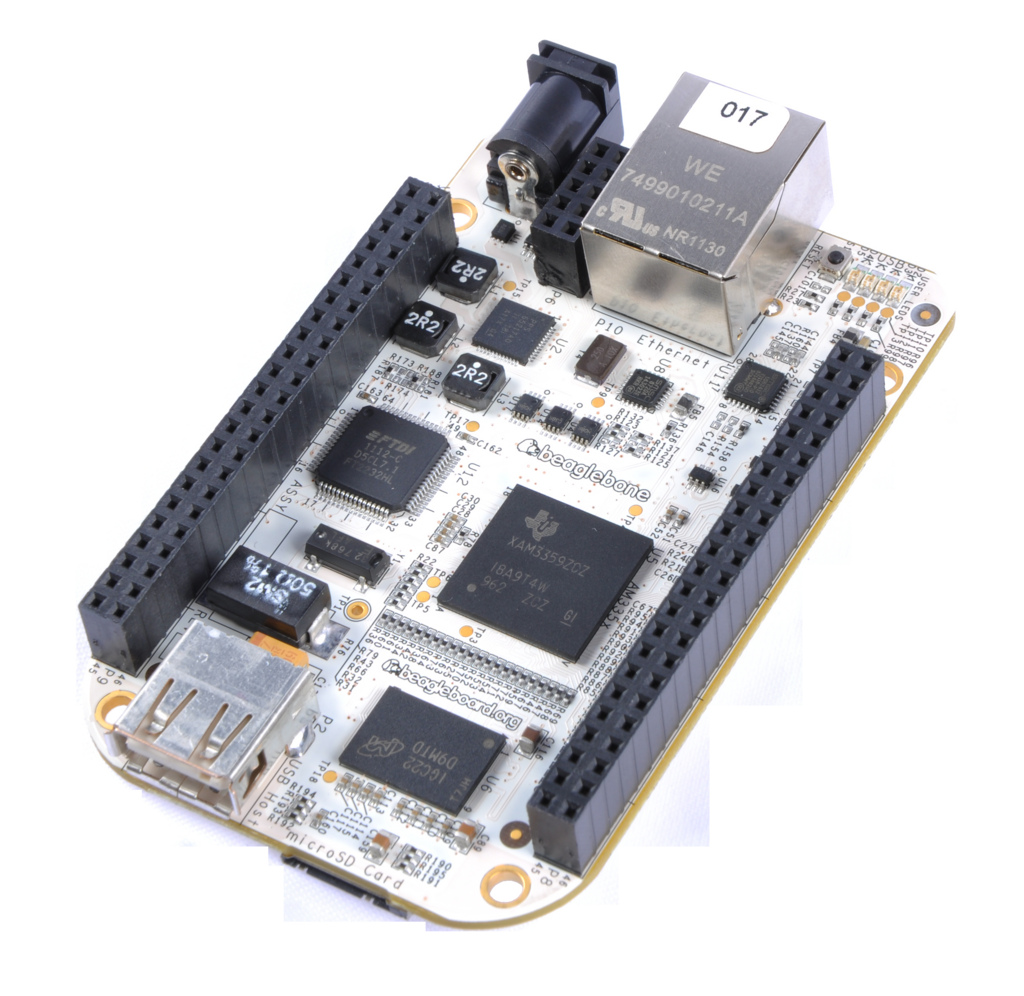
\includegraphics[scale=0.5]{img_beaglebone.jpg}
\end{columns}
\end{frame}

\section{Podsumowanie}

\begin{frame}
\frametitle{Podsuowanie}
\begin{itemize}
	\item NetBSD w zastosowaniach wbudowanych sprawdza się... etc.
\end{itemize}
\end{frame}


\begin{frame}
\frametitle{Jeśli system NetBSD was zainteresował...}
\begin{itemize}
	\item Oficjalna strona NetBSD -- \href{http://www.NetBSD.org/}{www.NetBSD.org}
\end{itemize}
\end{frame}

\begin{frame}
\frametitle{Pytania}

\begin{itemize}
	\item Czy są jakieś pytania?
\end{itemize}
\end{frame}

\begin{frame}
\frametitle{Koniec\ldots}
\vspace*{-0.8cm}
\begin{center}

\includegraphics[scale=0.5]{NetBSD.png}

Dziękuje!
\end{center}
\end{frame}

 
\end{document}
